%%%%%%%%%%%%%%%%%%%%%%%%%%%%%%%%%%%%%%%%%
% "ModernCV" CV and Cover Letter
% LaTeX Template
% Version 1.11 (19/6/14)
%
% This template has been downloaded from:
% http://www.LaTeXTemplates.com
%
% Original author:
% Xavier Danaux (xdanaux@gmail.com)
%
% License:
% CC BY-NC-SA 3.0 (http://creativecommons.org/licenses/by-nc-sa/3.0/)
%
% Important note:
% This template requires the moderncv.cls and .sty files to be in the same 
% directory as this .tex file. These files provide the resume style and themes 
% used for structuring the document.
%
%%%%%%%%%%%%%%%%%%%%%%%%%%%%%%%%%%%%%%%%%

%----------------------------------------------------------------------------------------
%	PACKAGES AND OTHER DOCUMENT CONFIGURATIONS
%----------------------------------------------------------------------------------------

\documentclass[11pt,a4paper,sans]{moderncv} % Font sizes: 10, 11, or 12; paper sizes: a4paper, letterpaper, a5paper, legalpaper, executivepaper or landscape; font families: sans or roman

\usepackage[utf8]{inputenc}

\usepackage[export]{adjustbox}

\usepackage{multicol}

\moderncvstyle{casual} % CV theme - options include: 'casual' (default), 'classic', 'oldstyle' and 'banking'
\moderncvcolor{blue} % CV color - options include: 'blue' (default), 'orange', 'green', 'red', 'purple', 'grey' and 'black'

\usepackage{color}

\usepackage{lipsum} % Used for inserting dummy 'Lorem ipsum' text into the template

\usepackage[scale=0.90]{geometry} % Reduce document margins
\setlength{\hintscolumnwidth}{4cm} % Uncomment to change the width of the dates column
%\setlength{\makecvtitlenamewidth}{10cm} % For the 'classic' style, uncomment to adjust the width of the space allocated to your name

%----------------------------------------------------------------------------------------
%	NAME AND CONTACT INFORMATION SECTION
%----------------------------------------------------------------------------------------

\firstname{dfdfds} % Your first name
\familyname{df} % Your last name

% All information in this block is optional, comment out any lines you don't need
\title{Curriculum Vitae}
%\address{14, Gonghangdae-ro 57gil, Gangseo-gu, Seoul, Republic of Korea}
%\mobile{+82 10 8635 3011}
%\phone{(000) 111 1112}
%\fax{(000) 111 1113}
%\email{jayeon0724@gmail.com}
%\homepage{staff.org.edu/~jsmith}{staff.org.edu/$\sim$jsmith} % The first argument is the url for the clickable link, the second argument is the url displayed in the template - this allows special characters to be displayed such as the tilde in this example
%\extrainfo{additional information}
%\photo[70pt][0.4pt]{pictures/picture} % The first bracket is the picture height, the second is the thickness of the frame around the picture (0pt for no frame)
%\quote{}

%----------------------------------------------------------------------------------------

\begin{document}

\textit{\Huge{\textcolor{gray}{Curriculum Vitae}}}

\hrulefill
%----------------------------------------------------------------------------------------
%	PERSONAL SECTION
%----------------------------------------------------------------------------------------

\begin{multicols}{2}
  \section{Personal Information}
  \cvitem{Name}{dfdfds df}
  \cvitem{Date of Birth}{\emph{dsf}}
  \cvitem{Address}{df}
  \cvitem{Mobile}{dfdf}
  \cvitem{Email}{dsfdf}
  \columnbreak
  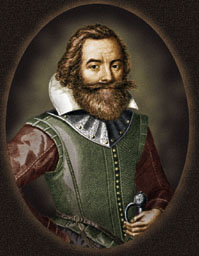
\includegraphics[width=28mm, right]{pictures/picture.jpg}
\end{multicols}

%\section{Presentation}
%\cvitem{}{I'm a Computer Science Engineer with specialization in Software Engineer graduated from Facultat d'Informàtica de Barcelona (UPC). I have 3 years of experience as Java back-end software engineer, both in design/planification and implementation tasks in different international projects at the university, working alongside companies and other universities. I also have some basic experience in front-end development tools. As a freelance developer, I'm currently working in two mobile app projects, and I have some experience in web development as well.}

%----------------------------------------------------------------------------------------
%	EDUCATION SECTION
%----------------------------------------------------------------------------------------
ObrazovanjeKorisnika


%----------------------------------------------------------------------------------------
%	WORK EXPERIENCE SECTION
%----------------------------------------------------------------------------------------


%----------------------------------------------------------------------------------------
%	EXTRACURRICULAR SECTION
%----------------------------------------------------------------------------------------
volonterskiRadIliProjekat
\

%----------------------------------------------------------------------------------------
%	SKILLS SECTION
%----------------------------------------------------------------------------------------
%\vspace{14mm}
\section{Skills \& Background Knowledge}

\subsection{Technical skills}

\cvitem{}{profVestina, \textit{nivo}}

%----------------------------------------------------------------------------------------
%	COMMUNICATION SKILLS SECTION
%----------------------------------------------------------------------------------------

\subsection{Personal skills}

\cvitem{}{vestina}

%----------------------------------------------------------------------------------------
%	LANGUAGES SECTION
%----------------------------------------------------------------------------------------

\section{Languages}

\cvitem{}{Korean, \textit{Native}}{}
\cvitem{}{English, \textit{Intermediate}}{}

\end{document}
